\documentclass[12pt]{article}
\usepackage{amsmath}
\usepackage{graphicx}
\usepackage{float}
\usepackage{amssymb}
\usepackage{pgfplots}
\pgfplotsset{compat=1.18}
\newcommand{\tabref}[1]{Table~\ref{#1}}
\newcommand{\figref}[1]{Figure~\ref{#1}}
\providecommand{\abs}[1]{\left\vert#1\right\vert}

\begin{document}

\title{Discrete Assignment}
\author{Mohana Eppala\\ EE23BTECH11018}
\maketitle

\section*{Problem Statement}
Determine the AP whose third term is 16 and the 7th term exceeds the 5th term by 12. 
\section*{Solution}
\begin{table}[H]

\centering
\begin{tabular}{|c|c|c|}
        \hline
        \textbf{Parameter} & \textbf{Value} & \textbf{Description} \\
        \hline
        $x(6) - x(4)$ & 12 & 7th term exceeds 5th by 12 \\
        \hline
	$x(2)$ & 16 & Third term \\
	\hline
        $d$ & ? & Common difference \\
        \hline
        $x(0)$ & ? & First term of AP \\
	\hline
        $x(n)$ & $(x(0) + nd)u(n)$ & General term \\
        \hline
\end{tabular}
\caption{Input parameters table}
\label{tab:1}

\end{table}


From \tabref{tab:1}
\begin{align}
    x(0) +6d - x(0) - 4d &= 12 \\ \implies
    2d &= 12\\ \implies
    d &= 6
\end{align}
Also,
\begin{align}
     x(0) + 2d &= 16 \\ \implies
	x(0) + 2(6) &= 16 \\ \implies
	x(0) &= 4 \\
	\therefore x(n) &= 6n + 4 
\end{align}
From \tabref{tab:1}
\begin{align}
	X(z) &= x(0)  \frac{1}{1-z^{-1}} + d \frac{z^{-1}}{(1 - z^{-1})^2} \\
	&= 4 \frac{1}{1-z^{-1}} + 6 \frac{z^{-1}}{(1 - z^{-1})^2} \\
	&= \frac{4+2z^{-1}}{(1-z^{-1})^2} \quad \abs{z} > 1
\end{align}



\begin{figure}[H]
    \centering
    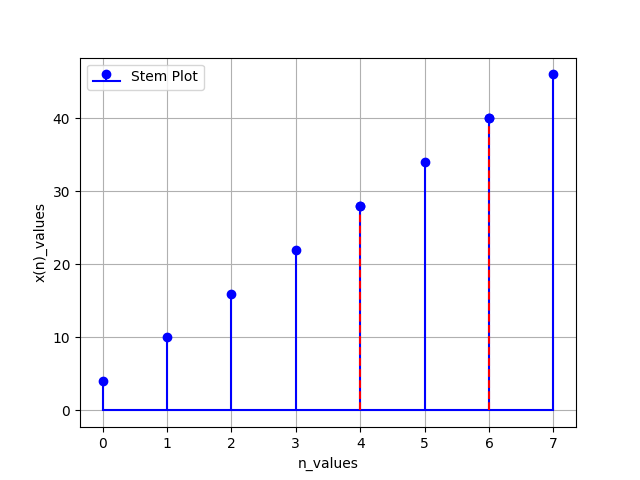
\includegraphics{figs/fig1.png}
    \caption{Given AP}
    \label{fig}
\end{figure}

\end{document}

